\documentclass[paper=a4,11pt,titlepage,twoside=true,headings=normal,numbers=noenddot,captions=tableabove,listof=totoc,index=totoc,bibliography=totoc]{scrreprt} % chapter erlaubt

% Language and Font Encoding
\usepackage{microtype}
\usepackage[ngerman]{babel}
\usepackage[T1]{fontenc} 
\usepackage[utf8]{inputenc}  % Remove if using XeLaTeX or LuaLaTeX
\usepackage{scrhack} 

% Math Packages
\usepackage{amssymb}
\usepackage[fleqn,intlimits]{amsmath} % [fleqn] for left-aligned equations

% Graphics and Tables
\usepackage{graphicx}
\usepackage[table]{xcolor}
\usepackage{booktabs}
\usepackage{multirow}
\usepackage{longtable}
\usepackage{tabularx}
\usepackage{tabulary}
\usepackage{float} % Improved control over float positioning
\usepackage{wrapfig} % Wrapping text around figures
\usepackage{rotating} % Rotating figures and tables

% Captions
\usepackage[labelfont={footnotesize,sf,bf},textfont={footnotesize,sf}]{caption}
\usepackage[font={scriptsize,sl},captionskip=3pt]{subfig}

% Units and Chemistry
\usepackage[locale=DE,per-mode=symbol]{siunitx} % For consistent SI units
\usepackage[version=4]{mhchem} % For chemical formulas

% Fonts and Typography
\usepackage{lmodern} % Improved font with better hyphenation support
\usepackage{csquotes} % Quotation handling
\usepackage{ellipsis} % Improved ellipsis handling

% Listings and Code
%\usepackage{listings}
\usepackage{minted}

% Hyperlinks
\usepackage{hyperref} % Must be loaded last
\hypersetup{
    linkcolor={0 1 1}, 
    linkbordercolor={1 1 1}, 
    citebordercolor={1 1 1},
    breaklinks=true,
    hidelinks
}

% Grafiken und Schaltkreise
\usepackage{tikz}
\usepackage{circuitikz}

% BIBlatex
\usepackage[backend=biber,style=phys,biblabel=brackets,defernumbers=true]{biblatex}
\usepackage[acronym]{glossaries}

% Sonstiges
\usepackage{lipsum} % Dummy Text zum Testen
%------------------ Schrifttyp in der Kopf- und Fußzeilen
\setkomafont{pageheadfoot}{\footnotesize\sffamily}

% Ändern der Abbildungs- und Tabellenbezeichnung (Niedermair S.157)
\addto\captionsngerman{\renewcommand\figurename{Abb.}}
\addto\captionsngerman{\renewcommand\tablename{Tab.}}
\renewcommand\listfigurename{Abbildungen}

% Betrag eines Wertes
\newcommand{\abs}[1]{\lvert #1 \rvert} 

% Absatz mit Formatierung
\newcommand{\absatz}[1]{\textbf{\textsc{#1}}} 

% Anhang Verweis
\newcommand{\anhang}[1]{Anhang \vref{#1}}

% Aufgabe Zähler
\newcommand{\aufgabe}{\stepcounter{plus} Aufgabe \arabic{plus}}

% Itemize Abkürzungen
\newcommand{\bi}{\begin{itemize}}
\newcommand{\ei}{\end{itemize}}

% Compact Enumerate Abkürzungen
\newcommand{\bce}{\begin{compactenum}}
\newcommand{\ece}{\end{compactenum}}

% Begin und End Equation
\newcommand{\be}{\begin{equation}}
\newcommand{\ee}{\end{equation}}

% Realteil einer Zahl
\newcommand{\real}[1]{\text{Re}\left\{#1\right\}}

% Multicolumn für Tabellen
\newcommand{\mc}{\multicolumn}

% Paralleltext
\newcommand{\pl}[1]{\ParallelLText{#1}}
\newcommand{\pr}[1]{\ParallelRText{#1}}
\newcommand{\pp}{\ParallelPar}

% Text in Rot
\newcommand{\textrot}[1]{\textcolor{red}{#1}}

% Abkürzung für multicolumn
\newcommand{\tab}[2]{\multicolumn{1}{#1}{#2}}

% Unterstreichen
\newcommand{\ul}[1]{\underline{#1}}

% Vspace Abkürzung
\newcommand{\vsf}{\vspace{5pt}}

% Abkürzungen für häufig verwendete Begriffe
\newcommand{\zb}{z.B.\,}
\newcommand{\idr}{i.d.R.\,}

% Zähler für Beispiele
\newcounter{req}
\newcommand{\zaehler}[1]{\refstepcounter{req}{#1} \thereq}






% Use geometry package for page layout settings
\usepackage[a4paper, left=3cm, right=3cm, top=3cm, bottom=3cm]{geometry}

% Set no indentation for paragraphs
\setlength{\parindent}{0cm}

% Set space between header and text
\setlength{\headsep}{20pt}

% Use scrlayer-scrpage for header and footer settings (KOMA-Script)
\usepackage{scrlayer-scrpage}
\clearpairofpagestyles
\ihead{\headmark}
\ofoot{\pagemark}
\setkomafont{pageheadfoot}{\footnotesize\sffamily}

\KOMAoptions{headsepline=.3pt:1\textwidth, footsepline=.2pt:1\textwidth}

% Einstellungen für Kopf- und Fußzeilen mit scrlayer-scrpage (KOMA-Script)
\usepackage{scrlayer-scrpage}
\pagestyle{scrheadings}

% Automatische Markierung von Kapiteln
\automark[chapter]{chapter}

% Kopfzeilen-Einstellungen
\ihead[]{Thema Bachelorarbeit} % Kopfzeile innen
\chead[]{} % Kopfzeile mittig
\ohead[]{\headmark} % Kopfzeile außen (Titel)

% Fußzeilen-Einstellungen
\ifoot[]{Max Mustermann} % Fußzeile innen (Name Autor)
\cfoot[]{} % Fußzeile mittig
\ofoot[]{\pagemark} % Fußzeile außen (Seitenzahl)


% Text für Kopf- und Fußzeilen

% Kopfzeile: Hochschule RheinMain auf ungeraden Seiten rechts, auf geraden Seiten links
% \newcommand{\titelkopfzeilelinks}{Hochschule RheinMain}
% \newcommand{\titelkopfzeilerechts}{Hochschule RheinMain}

% Fußzeile: Studienbereich auf ungeraden Seiten links, auf geraden Seiten rechts, Seitenzahlen in der jeweils anderen Position
% \newcommand{\titelfusszeilelinks}{Studienbereich Angewandte Physik \& Medizintechnik}
% \newcommand{\titelfusszeilerechts}{Seite \thepage\ von \pageref{LastPage}}

\makeglossaries

% Glossareinträge
\newglossaryentry{latex}{
    name={LaTeX},
    description={Ein Dokumentenmarkup-System, das häufig für wissenschaftliche Arbeiten verwendet wird}
}

\newglossaryentry{chatgpt}{
    name={ChatGPT},
    description={Ein generatives KI-Textmodell, das für Textverarbeitung und -generierung verwendet wird}
}

\newacronym{hsrm}{HSRM}{Hochschule RheinMain}

\usepackage{etoolbox}
\newbool{deutsch}
% \booltrue{deutsch}	% comment out to switch document to english

%---------------------------- VARIABLEN festlegen ------------------

%----------- TITEL
\newcommand{\titelLV}{Praktikumsbericht} % Bachelorarbeit, TitelLV, etc
\newcommand{\untertitela}{Berufspraktische Tätigkeit von\\[0.4cm] Max Mustermann} 
% Thema der Abschlussarbeit Ein prägnanter Haupttitel max. 1 Zeile ggf. ergänzt durch einen ausführlicheren Untertitel mit max: 2 Zeilen, max. 250 Zeichen gesamt] 

%---------- Studenten
% -------- Student 1
\newcommand{\nameA}{Matrikelnummer: 1234567} % Name
% --------- Student 2, falls vorhanden
\newcommand{\nameB}{}
% --------- Student 3, falls vorhanden
\newcommand{\nameC}{} %<--- Inhalt "Herr Student drei" bei Bedarf löschen

%---------- Datum einfügen
%\newcommand{\datum}{26.01.2021} % oder
\newcommand{\datum}{\today} %  aktuelles Datum

%----------- Lehrveranstaltungsleitung
\newcommand{\lvleitung}{Prof. Dr. Albert Einstein}

%----------------------------- Literaturdateien einfügen
\addbibresource{A-Literatur-Buecher.bib}
%\addbibresource{A-Literatur-Normen.bib}
\addbibresource{A-Literatur-Internet.bib}



%:::::::::::::::::::::::::::::::::::::::::::::::::::::::::::::::::::::::::::::::::::::::::::::::
\begin{document}
%:::::::::::::::::::::::::::::::::::::::::::::::::::::::::::::::::::::::::::::::::::::::::::::::

% Titelblatt einfügen
%\begin{titlepage}
    \newcommand{\HRule}{\rule{\linewidth}{0.5mm}}
    \centering
    \textsc{\Large Hochschule RheinMain \\
        
\includegraphics[width=0.15\textwidth]{logo-hsrm}\\[1cm]}
    
    \textsc{\LARGE \titelLV}\\[0.5cm]
    \HRule\\[0.4cm]
    {\huge\bfseries \untertitela}\\[0.6cm]
    \HRule\\[1.5cm] 
    
    % Author
    \large \textsc{\nameA}\\[0.5cm]

    % Supervisor and Department
    \vfill
    \textsc{\Large \lvleitung}\\[0.5cm]
    \textsc{\Large Fachbereich Ingenieurwissenschaften}\\[0.5cm]
    \textsc{\large Studienbereich Angewandte Physik \& Medizintechnik}\\[0.5cm]

    \vfill
    \hspace{0.4cm} {\large Datum der Berichtsabgabe: \datum}
\end{titlepage}
 % Laborprotokolle, Technische Berichte
\begin{titlepage}
    % Logo der Hochschule rechts oben einbinden
    \begin{minipage}[t]{\textwidth}
        \raggedleft
        
\includegraphics[width=0.4\textwidth]{logo-hsrm-2}%
    \end{minipage}\\[0.5cm]
    
    % Fachbereich und Studieninformationen
    \centering
    \textbf{Fachbereich Ingenieurwissenschaften}\\[0.5cm]
    \textbf{Studiengang Interdisziplinäre Ingenieurwissenschaften}\\[0.5cm]
    \textbf{Studienrichtung Medizintechnik}\\[1.5cm]

    % Titel der Arbeit
    \LARGE BACHELORARBEIT \\[2.5cm] % MASTERARBEIT
    \Huge \textbf{[Thema der Abschlussarbeit]}\\[0.5cm]
    \LARGE Irgendein Aussagekräftiger Untertitel der dieses Template näher beschreibt und maximal zwei Zeilen Lang ist \\[4cm] 
    % ggf. ergänzt durch einen ausführlicheren Untertitel mit max. 2 Zeilen, max. 250 Zeichen gesamt! 
    
    % Angabe zur Anfertigung
    \large Angefertigt: \textit{[im Labor ABC der Hochschule RheinMain, für Firma XYZ, Ort]}\\[2cm]
    
    % Autoreninformation (linksbündig)
    \raggedright
    Name: \textit{[Hans Mustermann]} \\[0.3cm]
    Matrikelnummer: \textit{[12345678]} \\[0.3cm]
    Referent/-in: \textit{[Prof. Dr. Eva Musterfrau]} \\[0.3cm]
    Korreferent/-in: \textit{[Dipl. Ing. Micha Müller]} 

    % Ort und Datum der Abgabe
    \centering
    \vfill
    Rüsselsheim, [DATUM]
\end{titlepage}
 % Thesis (unter 6b ausfüllen!)

%-----------------------------------------------------
\pagenumbering{roman}

% Versicherung, Abstract, Danksagung
% VERSICHERUNG
% ---------------------------------------------------------
\chapter*{Versicherung}
Hiermit versichere ich, dass ich die vorliegende Arbeit selbständig und ohne unzulässige Hilfe Dritter verfasst haben. Die aus fremden Quellen direkt oder indirekt übernommenen Texte, Gedankengänge, Konzepte usw. in meinen Ausführungen habe ich als solche eindeutig gekennzeichnet und mit vollständigen Verweisen auf die jeweilige Urheberschaft und Quelle versehen.\\ \\ 
Zudem kam der Generative Pre-trained Transformer ChatGPT zum Einsatz, um die eigenständig recherchierten Informationen in einen klar verständlichen Text umzuformulieren. Verbesserungen am Text durch ChatGPT wurden nicht gesondert gekennzeichnet, wohingegen durch ChatGPT nach präziser Anweisung generierte Textpassagen stets als solche markiert wurden.\\ \\
Mir ist bekannt, dass ein Täuschungsversuch vorliegt, wenn sich eine der vorstehenden Versicherungen als unrichtig erweist.\\ \\
\\
Wiesbaden, {\today} 
\\ 
\\
Ort, Datum und Unterschrift Verfasser
\newpage
% Gruppenarbeiten
% Hiermit versichern wir, dass wir die vorliegende Arbeit selbständig und ohne unzulässige Hilfe Dritter verfasst haben. Die aus fremden Quellen direkt oder indirekt übernommenen Texte, Gedankengänge, Konzepte usw. in unseren Ausführungen haben wir als solche eindeutig gekennzeichnet und mit vollständigen Verweisen auf die jeweilige Urheberschaft und Quelle versehen.\ \ Zudem kam der Generative Pre-trained Transformer ChatGPT zum Einsatz, um die eigenständig recherchierten Informationen in einen klar verständlichen Text umzuformulieren. Verbesserungen am Text durch ChatGPT wurden nicht gesondert gekennzeichnet, wohingegen durch ChatGPT nach präziser Anweisung generierte Textpassagen stets als solche markiert wurden.\ \ Uns ist bekannt, dass ein Täuschungsversuch vorliegt, wenn sich eine der vorstehenden Versicherungen als unrichtig erweist.\ \

% ABSTRACT
% ---------------------------------------------------------
\chapter*{Abstract}
Die vorliegende Arbeit untersucht die Optimierung von Mikrofluidiksystemen zur Anwendung in der medizinischen Diagnostik. Ziel der Arbeit ist es, die Effizienz des Probentransports in mikrofluidischen Chips zu verbessern, indem verschiedene Geometrien und Oberflächenbehandlungen verglichen werden. Zu diesem Zweck wurden sowohl numerische Simulationen als auch Laborversuche durchgeführt. Die Ergebnisse zeigen, dass eine spezielle Modifikation der Kanäle zu einer deutlichen Reduktion des Flüssigkeitswiderstandes und damit zu einer schnelleren Probentransportzeit führt. Diese Erkenntnisse tragen zur Weiterentwicklung effizienter und kostengünstiger Lab-on-a-Chip-Technologien bei, die für die schnelle medizinische Diagnostik von großem Interesse sind.
% Der Abstract ist eine kompakte Zusammenfassung der gesamten Arbeit. Er ist oft das Erste, was Leser oder Gutachter sehen, und sollte ihnen eine klare Vorstellung vom Inhalt und den Ergebnissen der Arbeit geben. Ein Abstract ist in der Regel zwischen 150-300 Wörtern lang.
% Inhalt des Abstract
% - Problemstellung: Was ist die zentrale Fragestellung oder das Problem, das die Arbeit adressiert?
% - Zielsetzung: Was soll erreicht werden?
% - Methoden: Welche Methoden wurden angewandt?
% - Ergebnisse: Was sind die wichtigsten Erkenntnisse oder Ergebnisse?
% - Schlussfolgerung: Welche Bedeutung haben die Ergebnisse?
\newpage


% ACKNOWLEDGEMENTS
% ---------------------------------------------------------
\chapter*{Danksagung}
Ich möchte mich herzlich bei meinem Betreuer Prof. Dr. Müller für die kompetente Betreuung und seine wertvollen Anregungen während der Erstellung dieser Arbeit bedanken. Ebenso danke ich meinen Kommilitonen, insbesondere Anna und Peter, für die zahlreichen konstruktiven Diskussionen und ihr hilfreiches Feedback. \\
Ein besonderer Dank gilt meiner Familie, die mich während des gesamten Studiums stets unterstützt hat und mir den Rücken freigehalten hat. Ohne ihre Ermutigung wäre diese Arbeit in dieser Form nicht möglich gewesen. \\
Zudem danke ich der Laborgruppe der XYZ Universität für die Bereitstellung der Laborinfrastruktur, die für die Durchführung der Experimente erforderlich war. \\
% Die Danksagung ist optional, wird aber häufig verwendet, um den Personen, Institutionen oder Organisationen zu danken, die die Arbeit unterstützt haben. Sie ist oft emotionaler als der Rest der Arbeit und dient dazu, die persönlichen Verbindungen und Unterstützungen zu würdigen, die zur erfolgreichen Durchführung der Arbeit beigetragen haben.
% Inhalt der Danksagung
% - Betreuer und wissenschaftliche Unterstützung: Dank an die Betreuer oder Dozenten, die fachlich unterstützt haben.
% - Kollegen und Mitstudierende: Dank an Kollegen, die vielleicht durch Feedback, Diskussionen oder Zusammenarbeit geholfen haben.
% - Familie und Freunde: Dank an die Familie und Freunde, die emotionale Unterstützung und Motivation gegeben haben.
% - Institutionen oder Förderer: Dank an Institutionen oder Programme, die eine finanzielle oder materielle Unterstützung bereitgestellt haben.
\newpage


% Inhaltsverzeichnis einfügen
\tableofcontents
\newpage

% Glossar einfügen
\printglossaries

%--------------------
\pagenumbering{arabic}
\setcounter{page}{1}

%-------------------------------------------------------------------------------------------------
%-------------------------------------------------------------------------------------------------
\chapter{Einleitung}
%-------------------------------------------------------------------------------------------------
%-------------------------------------------------------------------------------------------------

% Die Einleitung ist der Einstieg in das Thema der Arbeit. Hier erklärst du den Hintergrund, das Thema, die Problemstellung und die Motivation für die Arbeit. Die Einleitung sollte auch die Zielsetzung der Arbeit klar formulieren und einen Überblick über die Struktur der Arbeit bieten.
% Bestandteile der Einleitung:
% - Hintergrund und Motivation
% - Problemstellung
% - Ziel der Arbeit
% - Kurzer Überblick über die Kapitelstruktur

\lipsum[1-14] % Beispieltext

 
\chapter{Theoretische Grundlagen}
%-------------------------------------------------------------------------------------------------

% - Hier werden die relevanten Theorien und Modelle beschrieben, die für das Verständnis der Arbeit notwendig sind.
% - Falls du auf bestehende wissenschaftliche Literatur zurückgreifst, solltest du diese hier zusammenfassen und die wichtigsten Konzepte erläutern.

%-------------------------------------------------------------------------------------------------
\section{Glosar und Akronyme}
%-------------------------------------------------------------------------------------------------
%-------------------------------------------------------------------------------------------------

\gls{latex} ist ein leistungsfähiges Werkzeug zum Setzen von wissenschaftlichen Arbeiten.
In dieser Arbeit wird \gls{latex} verwendet, um das Dokument zu erstellen. Außerdem kam \gls{chatgpt} zum Einsatz, um Texte zu verbessern. Die \acrshort{hsrm} bietet eine Vielzahl an technischen Studiengängen. 
Die \acrshort{hsrm} ist bekannt für ihre technischen Studiengänge. Die \acrfull{hsrm} bietet viele Möglichkeiten für Forschung und Lehre.



%-------------------------------------------------------------------------------------------------
\section{Zitieren}
%-------------------------------------------------------------------------------------------------
%-------------------------------------------------------------------------------------------------

Hier schreiben Sie den Text für Ihr Thema hinein.

sfas \cite{ChatGPTl} \cite{Richard.2020} \cite{Fushimi.Mehrzyklone} \cite{Schlegel.MedPhy.2018}

In wissenschaftlichen Arbeiten ist es wichtig, die verwendeten Quellen korrekt zu zitieren. Hier sind einige Beispiele, wie man nach dem IEEE-Stil zitiert:

\begin{itemize}
    \item \textbf{Einfaches Zitat}: Ein einfaches Zitat mit einer Nummer in eckigen Klammern: \cite{ChatGPTl}. Dies ist der übliche Stil nach IEEE.
    \item \textbf{Mehrere Quellen}: Es ist auch möglich, mehrere Quellen gleichzeitig zu zitieren: \cite{Richard.2020, Fushimi.Mehrzyklone}. Die Zitate werden automatisch nummeriert.
\end{itemize}

Zusätzlich wird im IEEE-Stil oft eine nummerierte Liste im Literaturverzeichnis verwendet, um alle Quellen aufzulisten. Achten Sie darauf, die Nummerierung konsistent zu halten.

Weitere Hinweise:
- Im IEEE-Stil werden die Autoren in der Reihenfolge des Erscheinens zitiert.
- Stellen Sie sicher, dass alle verwendeten Quellen auch im Literaturverzeichnis aufgelistet sind.


%-------------------------------------------------------------------------------------------------
\section{Abbildungen}
%-------------------------------------------------------------------------------------------------
%-------------------------------------------------------------------------------------------------

\begin{figure}[H]
    \centering
    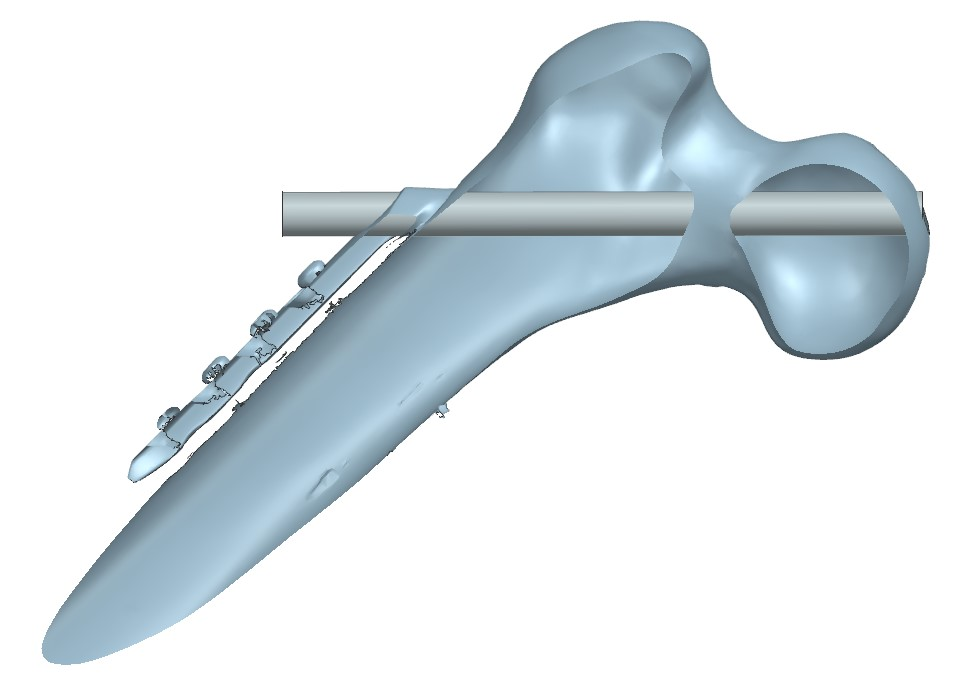
\includegraphics[width=0.6\textwidth]{abb1/bohrschablone_Seitenansicht.jpg} % Anpassung der Breite des Bildes
    \caption{Bohrschablone \cite{ChatGPTl}}
    \label{bild groß}
\end{figure}



\begin{figure}[H]
    \centering
    \begin{minipage}{0.4\textwidth}
        \centering
        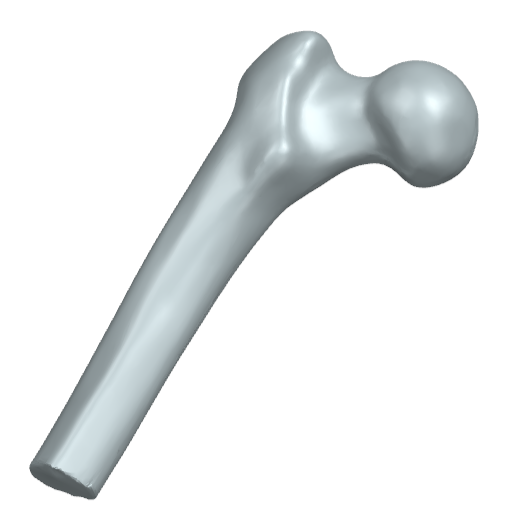
\includegraphics[width=\textwidth]{abb1/Femur_oben_GOM.png}
        \caption{einstein Bodybuilding}
        \label{fig:bildMitText}
    \end{minipage}
    \hfill
    \begin{minipage}{0.55\textwidth}
        \textbf{Beschreibung:}\\
        Dies ist ein Beispiel für einen Textabschnitt neben einem Bild. Hier können Sie eine ausführliche Beschreibung des Bildes oder andere relevante Informationen hinzufügen.
    \end{minipage}
\end{figure}



\begin{figure}[H]
    \centering
    \begin{minipage}[b]{0.3\textwidth}
        \centering
        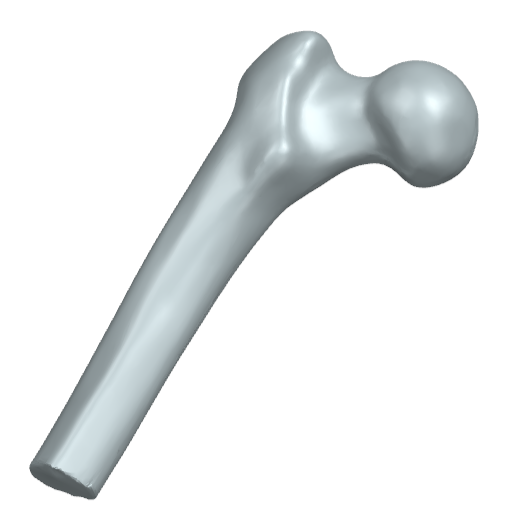
\includegraphics[width=\textwidth]{abb1/Femur_oben_GOM.png}
        \caption{Bild 1}
    \end{minipage}
    \hfill
    \begin{minipage}[b]{0.3\textwidth}
        \centering
        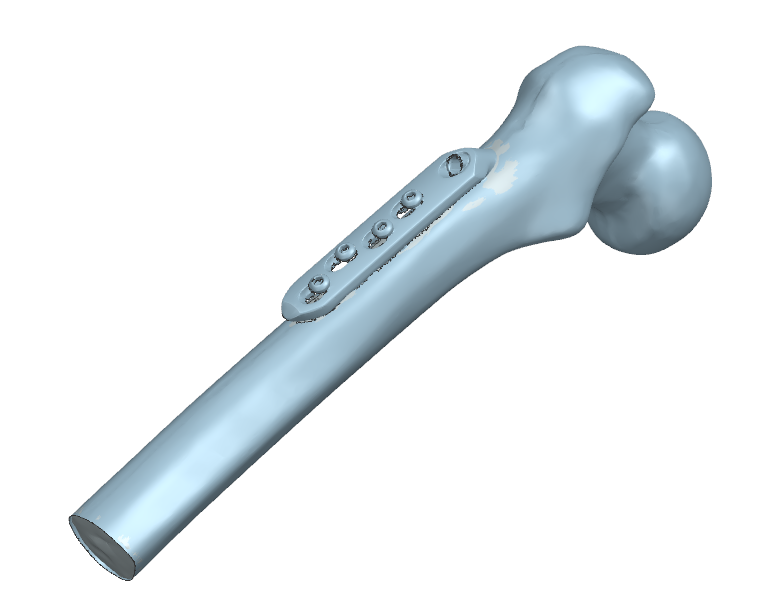
\includegraphics[width=\textwidth]{abb1/Impl_2_3D_Scan.png}
        \caption{Bild 2}
    \end{minipage}
    \hfill
    \begin{minipage}[b]{0.3\textwidth}
        \centering
        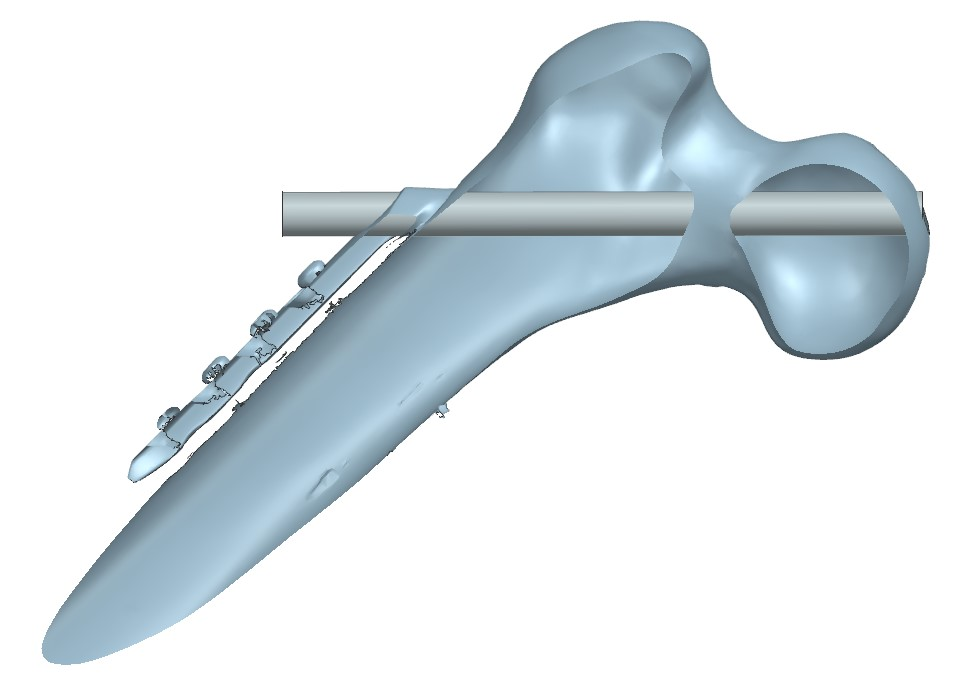
\includegraphics[width=\textwidth]{abb1/bohrschablone_Seitenansicht.jpg}
        \caption{Bild 3}
    \end{minipage}
\end{figure}



%-------------------------------------------------------------------------------------------------
\section{Tabellen}
%-------------------------------------------------------------------------------------------------
%-------------------------------------------------------------------------------------------------

\textbf{TABELLEN HABEN ÜBERSCHRIFTEN UND BILDER HABEN UNTERSCHRIFTEN!!!}

% Tabelle mit Vergleich zwischen Katzen und Raben
\begin{table}[H]
    \centering
    \caption{Vergleich zwischen Katzen und Raben}
    \begin{tabular}{|c|c|c|}
        \hline
        \textbf{Eigenschaft} & \textbf{Katzen} & \textbf{Raben} \\
        \hline
        Lebensdauer & 12-18 Jahre & 10-15 Jahre \\
        \hline
        Gewicht & 4-5 kg & 0.7-1.4 kg \\
        \hline
        Nahrung & Fleischfresser & Allesfresser \\
        \hline
        Lebensraum & Haushalte, Wildnis & Wälder, Städte \\
        \hline
        Intelligenz & Hoch & Sehr hoch \\
        \hline
        Soziales Verhalten & Einzelgänger & Gesellig \\
        \hline
    \end{tabular}
    \label{tab:katzen_raben}
\end{table}


\begin{table}[H]
    \centering
    \caption{Bilder in Tabellen}
    \begin{tabular}{c c c}
        \hline
        \textbf{Abbildung 1} & \textbf{Noch ein weiteres Bild} \\
        \hline
            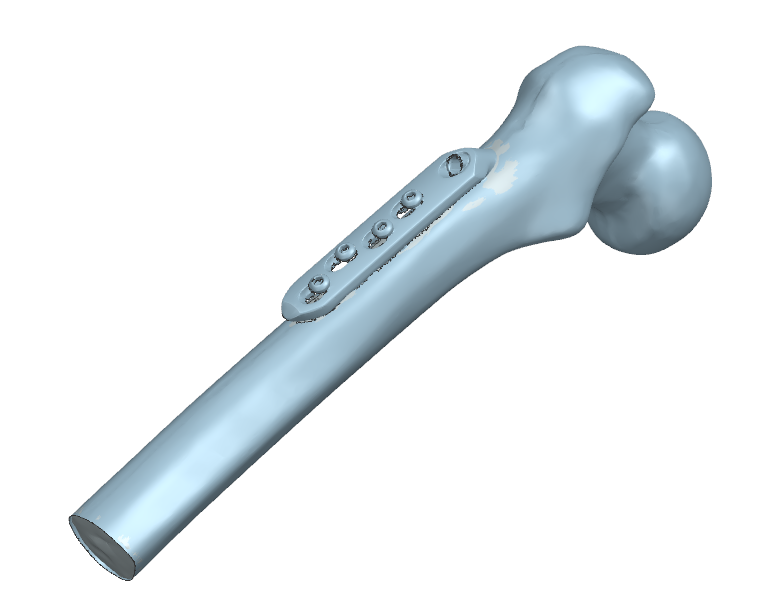
\includegraphics[width=0.2\linewidth]{abb1/Impl_2_3D_Scan.png} & 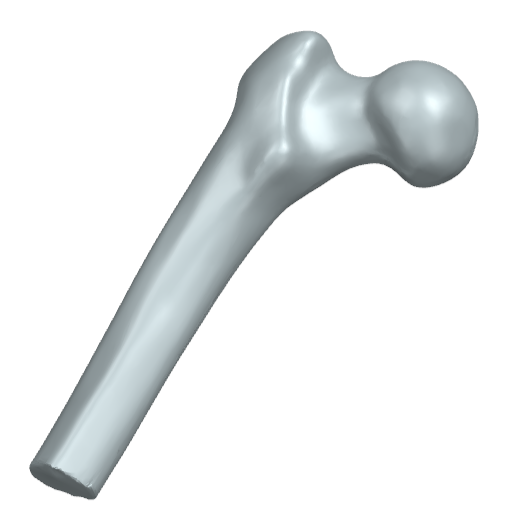
\includegraphics[width=0.2\linewidth]{abb1/Femur_oben_GOM.png} \\ 
        \hline
    \end{tabular}
    \label{BilderTab}
\end{table}


% Tabelle ohne Rahmen
\begin{table}[H]
    \centering
    \caption{Vergleich zwischen Katzen und Raben}
    \begin{tabular}{ c c c }
        \textbf{Eigenschaft} & \textbf{Katzen} & \textbf{Raben} \\
        Lebensdauer & 12-18 Jahre & 10-15 Jahre \\
        Gewicht & 4-5 kg & 0.7-1.4 kg \\
        Nahrung & Fleischfresser & Allesfresser \\
        Lebensraum & Haushalte, Wildnis & Wälder, Städte \\
        Intelligenz & Hoch & Sehr hoch \\
        Soziales Verhalten & Einzelgänger & Gesellig \\
    \end{tabular}
    \label{ohneRahmenTab}
\end{table}


% Tabelle mit nur einem Feld, das ein Bild enthält
\begin{table}[H]
    \centering
    \caption{Tabelle mit nur einem Feld, das ein Bild enthält}
    \begin{tabular}{c}
        \includegraphics[width=0.8\textwidth]{abb1/Gegenüberstellungsmatrix.png} % Pfad zum Bild anpassen
    \end{tabular}
    \label{tab:einBild}
\end{table}


%-------------------------------------------------------------------------------------------------
\section{Mathematisches}
%-------------------------------------------------------------------------------------------------

Hier schreiben Sie den Text für Ihr Thema hinein.

% Einfache Formel im Text
Die berühmte Einstein-Gleichung ist $E = mc^2$.

% Abgesetzte Formel ohne Nummer
\[
E = mc^2 
\]

% Abgesetzte Formel mit Nummer
\begin{equation}
E = mc^2
\label{einstein.eq}
\end{equation}

Gleichung \ref{einstein.eq} ist Einsteins Gleichung.

% Mehrzeilige Formel (Millikan-Versuch)
\begin{align}
q &= ne \\
F &= qE \\
ma &= qE \\
a &= \frac{qE}{m}
\end{align}

% Formel mit Summen und Integralen
\begin{equation}
\int_0^\infty e^{-x^2} \, dx = \frac{\sqrt{\pi}}{2}
\end{equation}

\[
i\hbar \frac{\partial}{\partial t} \Psi(\mathbf{r}, t) = \hat{H} \Psi(\mathbf{r}, t)
\]

% Formel mit Brüchen
\begin{equation}
f(x) = \frac{a}{b} + \frac{c}{d}
\label{eq2}
\end{equation}

% Formel mit griechischen Buchstaben und Exponenten
\begin{equation}
\alpha^2 + \beta^2 = \gamma^2
\label{eq1}
\end{equation}

% Erweiterte Mathematische Beispiele
\begin{equation}
\nabla \times \mathbf{E} = -\frac{\partial \mathbf{B}}{\partial t}
\label{maxwell1}
\end{equation}

\begin{equation}
\oint_\mathcal{C} \mathbf{B} \cdot d\mathbf{l} = \mu_0 I + \mu_0 \epsilon_0 \frac{d\Phi_E}{dt}
\label{maxwell2}
\end{equation}

Hier kann man auch auf Gleichungen verweisen! Gleichungen \ref{maxwell1} und \ref{maxwell2} sind Teil der Maxwell-Gleichungen.

%-------------------------------------------------------------------------------------------------
\section{Code Beispiele}
%-------------------------------------------------------------------------------------------------

\subsection{Python Code}
\begin{minted}[linenos, fontsize=\small]{python}
def fibonacci(n):
    """Berechnet die Fibonacci-Zahlen bis n."""
    a, b = 0, 1
    while a < n:
        print(a, end=' ')
        a, b = b, a + b
    print()
    
fibonacci(1000)
\end{minted}

\subsection{C++ Code}
\begin{minted}[linenos, fontsize=\small]{c++}
#include <iostream>

void fibonacci(int n) {
    int a = 0, b = 1;
    while (a < n) {
        std::cout << a << " ";
        int temp = a;
        a = b;
        b = temp + b;
    }
    std::cout << std::endl;
}

int main() {
    fibonacci(1000);
    return 0;
}
\end{minted}

%-------------------------------------------------------------------------------------------------
\section{Schaltkreise}
%-------------------------------------------------------------------------------------------------

Für Schaltkreise verwenden Sie das \texttt{circuitikz}-Paket:

\begin{figure}[H]
    \centering
    \begin{circuitikz}
        \draw (0,0) to[battery, l=9V] (0,2) to[resistor, l=R] (2,2) to[bulb, l=Glühbirne] (2,0) -- (0,0);
    \end{circuitikz}
    \caption{Ein einfacher Stromkreis mit Batterie, Widerstand und Glühbirne}
    \label{fig:stromkreis}
\end{figure}

%-------------------------------------------------------------------------------------------------
\section{Vektorgrafiken}
%-------------------------------------------------------------------------------------------------

Für Vektorgrafiken verwenden Sie das \texttt{tikz}-Paket:

\begin{figure}[H]
    \centering
    \begin{tikzpicture}
        % Erstellen eines einfachen Hauses
        \draw[thick] (0,0) rectangle (2,2); % Quadrat
        \draw[thick] (0,2) -- (1,3) -- (2,2); % Dach
        \draw (0.75,0) rectangle (1.25,1); % Tür
    \end{tikzpicture}
    \caption{Eine einfache Vektorgrafik: Haus}
    \label{fig:vektorgrafik}
\end{figure}



%-------------------------------------------------------------------------------------------------
\section{Aufzählungen und Listen}
%-------------------------------------------------------------------------------------------------

\subsection{Aufzählungen}
\begin{itemize}
  \item Punkt eins
  \item Punkt zwei
  \item Punkt drei
\end{itemize}

\subsection{Nummerierte Listen}
\begin{enumerate}
  \item Erster Punkt
  \item Zweiter Punkt
  \item Dritter Punkt
\end{enumerate}

\subsection{Verschachtelte Listen}
\begin{itemize}
  \item Erster Punkt
  \begin{itemize}
    \item Unterpunkt eins
    \item Unterpunkt zwei
  \end{itemize}
  \item Zweiter Punkt
\end{itemize}



   
%-------------------------------------------------------------------------------------------------
%-------------------------------------------------------------------------------------------------
\chapter{Material und Methoden}
%-------------------------------------------------------------------------------------------------
%-------------------------------------------------------------------------------------------------

% - Dieser Abschnitt beschreibt die Methodik, die für die Untersuchung verwendet wurde.
% - Es ist wichtig, hier sehr präzise zu sein, damit der Leser die Vorgehensweise nachvollziehen kann und die Ergebnisse reproduzierbar sind.
% - Falls spezifische Materialien, Software oder Hardware verwendet wurden, sollten diese auch genau beschrieben werden.



%-------------------------------------------------------------------------------------------------
\section{xyz}
%-------------------------------------------------------------------------------------------------
%-------------------------------------------------------------------------------------------------

asf


%-------------------------------------------------------------------------------------------------
\subsection{asdf}
%-------------------------------------------------------------------------------------------------

asfdsf

%-------------------------------------------------------------------------------------------------
\subsection{asdf}
%-------------------------------------------------------------------------------------------------

asdfsaf



%-------------------------------------------------------------------------------------------------
\section{xyz}
%-------------------------------------------------------------------------------------------------
%-------------------------------------------------------------------------------------------------

Fasfasdsa

 
%-------------------------------------------------------------------------------------------------
%-------------------------------------------------------------------------------------------------
\chapter{Ergebnisse}
%-------------------------------------------------------------------------------------------------
%-------------------------------------------------------------------------------------------------

% - Die Ergebnisse der Untersuchung werden in diesem Abschnitt dargestellt. Hier präsentierst du die Daten, die du während deiner Arbeit gesammelt hast.
% - Graphiken, Tabellen und andere Visualisierungen sind sehr nützlich, um die Ergebnisse verständlich darzustellen.
% - Wichtig ist es, die Ergebnisse möglichst objektiv und ohne Interpretation darzustellen.



%-------------------------------------------------------------------------------------------------
\section{xyz}
%-------------------------------------------------------------------------------------------------
%-------------------------------------------------------------------------------------------------

asf


%-------------------------------------------------------------------------------------------------
\subsection{asdf}
%-------------------------------------------------------------------------------------------------

asfdsf

%-------------------------------------------------------------------------------------------------
\subsection{asdf}
%-------------------------------------------------------------------------------------------------

asdfsaf



%-------------------------------------------------------------------------------------------------
\section{xyz}
%-------------------------------------------------------------------------------------------------
%-------------------------------------------------------------------------------------------------

Fasfasdsa

  
%-------------------------------------------------------------------------------------------------
%-------------------------------------------------------------------------------------------------
\chapter{Diskussion}
%-------------------------------------------------------------------------------------------------
%-------------------------------------------------------------------------------------------------

% - In der Diskussion setzt du dich kritisch mit den Ergebnissen auseinander.
% - Hier interpretierst du die Ergebnisse und setzt sie in den Kontext der Problemstellung.
% - Es ist wichtig, auch die Grenzen der Untersuchung anzusprechen und mögliche Fehlerquellen zu analysieren.

sfas



%-------------------------------------------------------------------------------------------------
\section{xyz}
%-------------------------------------------------------------------------------------------------
%-------------------------------------------------------------------------------------------------

asf


%-------------------------------------------------------------------------------------------------
\subsection{asdf}
%-------------------------------------------------------------------------------------------------

asfdsf

%-------------------------------------------------------------------------------------------------
\subsection{asdf}
%-------------------------------------------------------------------------------------------------

asdfsaf



%-------------------------------------------------------------------------------------------------
\section{xyz}
%-------------------------------------------------------------------------------------------------
%-------------------------------------------------------------------------------------------------

Fasfasdsa

   
%-------------------------------------------------------------------------------------------------
%-------------------------------------------------------------------------------------------------
\chapter{Schlussfolgerungen und Fazit}
%-------------------------------------------------------------------------------------------------
%-------------------------------------------------------------------------------------------------

% - Das Fazit zieht die Arbeit zusammen und gibt eine abschließende Bewertung der erzielten Ergebnisse.
% - Es ist wichtig, hier auch einen Ausblick auf mögliche weitere Untersuchungen zu geben. Dies zeigt, dass du über den Tellerrand hinausschaust und zukünftige Forschungsmöglichkeiten erkennst.











%-------------------
\newpage
\renewcommand{\refname}{Literatur- und Quellenverzeichnis} % bei scrartcl
\renewcommand{\bibname}{Literatur- und Quellenverzeichnis} % bei scrbook und scrrprt
\printbibheading
%\printbibliography[nottype=online,heading=subbibliography,
\printbibliography[type=book,heading=subbibliography,
title={Literaturverzeichnis}]
\printbibliography[type=online,heading=subbibliography,
title={Quellenverzeichnis (Internet)}]
%\printbibliography[type=misc,heading=subbibliography,
%title={Normenverzeichnis}]

%----------- Bild und Tabellenverzeichnis
\newpage
\listoffigures 
\listoftables
\newpage

\appendix
% Anhangsbeginn
% Inhaltsverzeichnis für den Anhang
\renewcommand{\thepage}{\Roman{page}} % Römische Seitenzahlen im Anhang
\pagenumbering{Roman} % Beginne mit römischen Ziffern

\chapter{Zusätzliche Materialien}
\lipsum[1-4]

\chapter{Experimentelle Daten}
\lipsum[5-8]

\chapter{Abkürzungen und Symbole}
\lipsum[9-17]

%:::::::::::::::::::::::::::::::::::::::::::::::::::::::::::::::::::::::::::::::::::::::::::::::
\end{document}
%:::::::::::::::::::::::::::::::::::::::::::::::::::::::::::::::::::::::::::::::::::::::::::::::